\subsection{Gaussian Processes}
Due to their seemingly simple nature and interesting analytical properties Gaussian processes have been used extensively in various tasks for centuries. Flexibility of Gaussian Processes have seen them employed in various forms. [BDA reference about 1800 century], Gelmen et al. mention them being used for astronomical data modelling in 18th century. Later, significant work have been done as part of stochastic process literature for example as Weiner processes and later for time series prediction[Weiner process, A Populi’91 reference for stochastic process and other Reference from Phd thesis]. In Spatial statistics, gaussian process regression was used for interpolation of values based on space as the input by Matheron in 1973 following the work of D.G. Krige [ both references from wiki]. In applied statistics context, Gaussian processes were first used for regression and classification [O’Hagan 1978], density estimation [reference from BDA, rihimaki thesis and other one ] etc. Inspired by the link shown between neural networks and Gaussian process by [Neal ‘ 96] Gaussian processes were quickly extended to machine learning context[Rasmussen 96]. With the advent of approximation schemes [Sparse approximation referneces] and hardware gains, use of Gaussian process has quickly skyrocketed in other areas of machine learning such as dimensionality reduction [reference], latent vector modelling [reference], even multi purpose deep Gaussian processes analogous to deep neural network have been proposed [GPRN paper, deep GP paper].  In the next few sections, we first define Gaussian processes and review it's properties like covariance functions etc briefly and later describe the inference procedure including  predictions and parameter selection in Section 2.2 
\subsubsection{Definition}
A function is generally thought of as a mapping from an arbitrary set X to another F(X), $X -> F(X)$. One interesting way to look at it can be of thinking X and F(X) as infinitely long vectors with former’s elements acting as an index for the latter, i.e. X as an index set for F(X).  A collection of these random mappings is called a process [Random Fields and geometry, Andler, Stochastic process book]. 

A Gaussian Process is thus formally defined as a collection of random variables, any finite set of which is jointly distributed. i.e. for a finite set x contained in X , collection of random variables F(x) will follow a Gaussian distribution [GPML book], i.e. 

\begin{equation}
    p(F|X) ~ mathbb{N}(m,K)
    \label{eqn:GP_definition}
\end{equation} 

In gaussian process terms f(x) is written as $f(x) ~ GP(m(x),k(x,x))$ where m(x) and k(x,x) are called the mean and covariance function respectively. 

\subsubsection{Covariance functions and Kernels}

From a function perspective, one expects that data points close/near to each other will have similar values. This notion of nearness can also be seen in general life for example, if one were to measure moisture in environment at a specific time every day for a year we expect days or places near each other to have similar temperatures. Gaussian Process represent this concept of nearness/closeness through a covariance function, i.e. how the function value changes with respect to the difference in their index values. Thus, a covariance function must take two indices and map them to a real number defining the correlation of underlying function’s values at the indices. 
The matrix K in equation \ref{eqn:GP_definition} is generated by applying this covariance function for each pair of elements in X. 
\begin{figure}
    \centering
    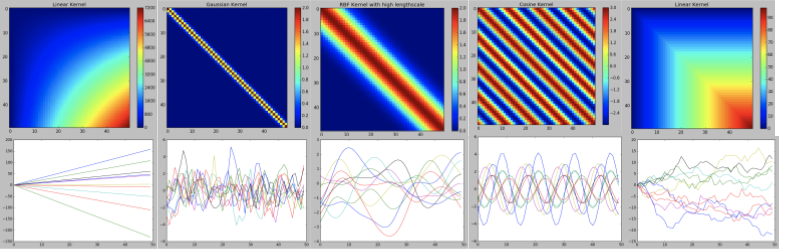
\includegraphics[scale=0.5]{thesis/images/Kernels_samples.png}
    \caption{Different Kernels and corresponding sampled GPs}
    \label{fig:generic_function_space}
\end{figure}

A covariance function, thus has two important responsibilities. First, when applied pairwise to the elements of set X it must be able to generate a proper covariance matrix (symmetric, positive semi definite etc.) and second, it should also somehow be a measure of nearness between two values, i.e. map its inputs to a real value. Former enables covariance function to significantly determine the properties of to be generated functions like smoothness, length-scale etc. from the corresponding GP to a large extent while latter means they are same as kernels of SVM literature [Kernel methods book ]

A Gaussian process is completely determined by its mean and co-variance function and once these two are fixed we can generate sample functions using equation \ref{eqn:GP_definition}  Fig 2.1: differnet covariance matrices and corresponding functions :  Shows A number of kernels and functions generated form corresponding  zero mean GPs. 

The mathematical literature on Gaussian process is quite extensive. [M Seeger’s paper and stochastic process book] are good references for detailed mathematical properties of GPs and of stochastic processes in general. [Bob 53, Grimment and Strizaker 1982> from OHagan book] are good references for application of GP in probability theory.

\subsubsection{Inference in GP}
Under Bayesian nonparametric framework, Gaussian processes are used to express our prior beliefs about underlying function that could describe observed data. By combining these prior assumptions with the observed information we arrive at the posterior representation of the latent function values.

A generic inference process of Gaussian process model which has n, Y ($[y_1,y_2,…y_n]$) values at locations X ($[x_1,x_2...x_n ]$) follows a hierarchical structure [Phd thesis RIhimaki]. 
First, we assume a data generating function $f_i = f(x_i)$ with n latent function values $f_1,f_2…f_n$ such that given these, Y’s are independent of locations X.
$$P(Y \mid F) = \Prod_{i=1}^{N}P(y_i \mid f_i)$$
The functional space from which these function values can arise is then constrained by putting a suitable GP prior over latent function values. $$ P(F(X) \mid \theta) = GP(m(X),K(X,X’ \mid \theta))$$
Finally, we can also put a prior over hyperparameters of covariance function, theta. 
	$$\theta ~ P(\theta)$$ 
Now, as explained in the section 2.2.2 a GP prior corresponds to a multivariate Gaussian distribution and hence prior for F can be written as:
$$P(F \mid X,\theta) = \mathbb{N}(F \mid 0, K_{xx})$$
Where $K_{xx}$ would be the covariance matrix generated through pairwise application of covariance function on observations X. Now following Bayesian inference rules the posterior can be obtained as,
\begin{equation}
P(F \mid X,Y,\theta) = \frac{P(Y \mid F)P(F \mid X, \theta)}{P(Y \mid X, \theta)} \approx \mathbb{N}(F \mid 0, K_{xx}) \prod_{i=1}^{n}P(y_i \mid f_i)
\label{eqn:GP_posterior}
\end{equation}

\subsubsection{Prediction}
Generally, we are also interested in the prediction of new latent values f* (or a new value y*) on different locations x*. In that case joint distribution of f and f* can be written as,
$$P(f,f^* \mid X,X*,y) ~ N([f, f*] | 0, [[K_{xx} K_{x*}],[K_{*x} K_{**}]])$$

Here $K_{x*}$ and $K_{**}$ are once again generated through pairwise application of covariance function on observed as well as new values and on new values respectively. $K_{x*}$ defines the covariance between new and observed function values while $K_{**}$ defines the covariance among new values.

Following conditional properties of Gaussian distribution [Bishop book, 87] we can generate distribution for f* given f as:
\begin{equation}
    P(f^* \mid f, X, x*) \approx \mathbb{N}(f^* \mid K_{*x}K_{xx}^{-1}f, K_{**} - K_{*x}K_{xx}^{-1}K_{x*} )
    \label{eqn:GP_prediction}
\end{equation}	 

Finally, if we are interested only in corresponding predicted values Y* it can be figured out as:
\begin{equation}
    P(y^* \mid Y, X, x*) \approx \Int P(y^* \mid f^*)P(f^* \mid X^*,Y,X)
\end{equation}
Here, $P(f^* \mid X^*,Y,X)$ is the posterior predictive distribution that can be obtained by integrating out the latent function values f from equation \ref{eqn:GP_prediction}

\subsubsection{Hyperparameter selection}

GP specifies a fully probabilistic model and hence it has a distinct advantage over other techniques that hyperparameters can be inferred from training data directly instead of using a cross validation scheme as in case of other methods. [luttinen’s thesis]
In a pure Bayesian framework, hyper-parameters would have priors set over them. However, complex relationship of hyper-parameters with covariance function means usually the integrals become intractable and must be done through other numerical methods like MCMC [W and R 2006] or likelihood maximization. Due to computational expensiveness of MCMC likelihood maximization is generally used for hyperparameter selection in GP. aA gradient based optimization procedure can be used thourgh Marginal data likelihood in the denominator of equation \ref{eqn:GP_posterior} to optimize hyperparameters,
$$P(Y \mid X, \theta) = \int P(Y \mid F)P(F \mid X, \theta) dF $$

Since the prior $P(F \mid X, \theta)$ is Gaussian ($\mathbb{N}(F \mid 0,K_{xx})$), after combining this with the Gaussian likelihood $P(Y \mid F) = \mathbb{N}(Y \mid F, \sigma^2)$ and integrating out F, the log marginal likelihood can be written as,

\begin{equation}
   log P(Y \mid X, \theta) = -\frac{1}{2}Y^{T}(K + \sigma^{2}I)^{-1}Y -\frac{1}{2} log (K + \sigma^{2}I) - \frac{n}{2} log \Pi
   \label{eqn:GP_likl}
\end{equation}

In the equation \ref{eqn:GP_likl} all the terms are a function of $\theta$. (K is calculated by pair wise application of function $k(\theta)$ on X) and hence optimal values of hyperparameters can be obtained by finding the gradient of  \ref{eqn:GP_likl} with respect to each $\theta_j \in \theta$

ML estimates might overfit sometimes however, a well peaked posterior drasitcally reduces overfitting risk of hyperparameters [Mackay 99]. 

\subsubsection{Regression using GP}
Gaussian process based Bayesian non parametric regression have been described in [Blight &Ott, hagan 1978, Neal 92] etc. The central idea is to first start with the parametric linear model and then generalize it through Gaussian processes. [W & R book] generalized regression by first using basis function to project standard linear regression to a high dimensional space and then using kernel trick [Kernel Methods book] to arrive at the same result as us section 2.2.3, this approach is also called the weight space view of Gaussian processes, details of which can be found in [oHagan 78, R & W book/paper , M Seeger]. 
Here we take a simpler approach based on the development of previous sections. Same equations can be arrived at using weight space view as illustrated in [http://dl.acm.org/citation.cfm?id=299093]
A generic regression problem can be defined as:
\begin{equation}
Y = f(x) + \epsilon(noise)
\label{eqn:regression}
\end{equation}
Where the objective is to find a good enough estimate of f(x) so that one could predict $Y^*$ values for input $X^*$. 
Traditional solution of the problem have been to use a parametric model similar to:
	$$F(x|w) = w_1 + w_2x + w_3x^2$$
Here w’s are also called the weights of the covariates. In Bayesian setting, w’s will be called the parameters and we put a prior p(w) on them. Once posterior $p(W \mid Y)$ is obtained we can predict new values using $p(Y^* \mid X^*, W)$. It can be observed that this approach quickly creates the problem of limiting the function capacity as explained in section 2.1. Moreover, it might also be difficult to encode prior beliefs about weights as a distribution p(W).

To provide an overly accommodating non linear functional space as prior for the desired regression function, we can put a Gaussian process prior over the weights. As explained in section 2.2 using GPs also alleviate the problem of providing our prior beliefs about parameters through covariance function and Kernels.

Thus the GP solution for regression problem in equation \ref{eqn:regression} becomes:

Prior: $P(f|X) = N(f| 0, K_{xx})$

where $K_xx$ is the covariance matrix for input X. 

We further assume Gaussian distribution for noise term in equation \ref{eqn:regression}:
	$$ \epsilon = N(0, \Sigma)$$
where $\Sigma = \sigma^2I$
Now following \ref{eqn:regression} likelihood of the observations is given by,

	$$ P(Y \mid F, X) = \mathbb{N}(f, \Sigma)$$

From here we can find the posterior in the similar way as in the section 2.3.2:
	
$$ P(f \mid X, Y) \approx \mathcal{N}(\mu_f, \S_f)$$

Here $\mu_f = (K_{xx}^{-1} + \Sigma^{-1})^{-1}\Sigma^{-1}Y$ and $S_f = (K_{xx}^{-1} + \Sigma^{-1})^{-1}$

Similarly, as in section Posterior predictive distribution for a new function value f* at point x* can be directly calculated using equation \ref{eqn:GP_prediction}

Regression is one of the simplest of Gaussian process use cases. [M seeger] provides pointers on to further generalize the model by allowing an arbitrary noise distribution directly in GP prior or extending it for other generalized linear models.  

\subsubsection{Classification using GP}
Classification is another common problem in machine learning in which desired functional value is categorical. In a generic classification setting, our observations include class labels Y ~ [1,2…M] corresponding to each data point X and our objective is to estimate a function F: X -> [1,2…M] that can assign the class labels appropriately to the new data points X* or in bayesian context finding the probability $P(y^* = c \mid x*, Y,X)$ where $c \in [1,2…M]$ 
The simplest case of GP classifier is called Bayesian discriminator [Ramsuseen Book, Barber and Williams] in which we consider a GP prior over the latent function and then the latent function values for data point are turned into class probabilities using a response function. This conversion of latent values of domain (–inf,+inf) to output of response function of domain (0,1) guarantees a valid probabilistic interpretation of our prediction. 
A common method to map the function values to probabilties is to use the logit function such that if y ~ {-1,1}  and $F_i$ is the latent function values for $X_i$:
	$$P(y_i \mid F_i)  = \sigma(y_i,f_i) = \frac{1}{(1+ exp^(-f_i))}$$

 Since the class labels are independent  from each other given latent function values, likelihood can be written as:
	$$ P(Y \mid F) = \Prod_(i=1)^{N} P(y_i \mid F_i) = \Prod_(i=1)^{N} \sigma(y_i,F_i)$$
	
Once again we put a GP prior on the latent function values $P(F \mid X) = \mathcal{GP}(F \mid \mu, K_{xx})$ and write the posterior as:
\begin{equation}
P(F \mid Y,X) = \frac{P(Y|F)P(F|X)}{P(Y \mid X)} = \frac{\mathcal{N}(F \mid 0, K_{xx})}{P(Y \mid X)}\Prod_{i=1}^{N}\sigma(y_i,F_i)
\end{equation}

Similarly, posterior predictive distribution of latent function is,
\begin{equation}
	P(F^* \mid X^*, Y,X) = \Int P(F^* \mid X^*, F ,X) p(F \mid X,Y) dF^*
\end{equation} 

Here $P(F^* \mid X^*, F ,X)$ is Gaussian that can be obtained through conditional GPs however, due to P(Y|F) and P(Y|X) being non Gaussian, both posterior and posterior predictive distribution become analytically intractable.
Since categorical predictions $y^*$ are much more important in classification context and we can still proceed for y* since we can integrate out the latent function values, 
$$P(y^*=+1 \mid X,Y,X^*) = \Int P(y* \mid F^*)P(F* \mid X,Y,X^*)dF^*$$

However, same as in previous case the integration is intractable and we must resort to approximation to obtain the distribution details. Section 2.3 describes variational inference scheme to find an approximation in the cases like this where an analytical  solution can not be obtained.
Apart from variational inference scheme described in next chapters, numerous other approximation solutions have been developed in for GP classification. An extensive survey of different approximation schemes for Classification using GPs can be found in  [http://mlg.eng.cam.ac.uk/pub/pdf/KusRas06.pdf] MOreover, Detailed treatment of more general cases of classification like multi-class classification or one class classification can be found in [Barber] and [http://hera.inf-cv.uni-jena.de:6680/pdf/Kemmler10:OCC.pdf] respectively.






